\section{Examples of usage}\label{sec:examples}
    The following chapters shows typical use-cases of \ac{scars} Toolbox. First two sections can serve the purpose of teaching with step-by-step instructions how to set-up a simple project. Following parts showcase real life example spacecrafts, which \ac{aocs} Subsystems can be simulated as accordingly set up \ac{scars} Modular Simulations. Finally, examples of control system tests are shown, proving that \ac{scars} can be used for both prototyping and reviewing processes.

    % \subsection{Initial set-up of ADCS architecture in SCARS}
        % \dots\textit{description}\dots

    \subsection{Simple spacecraft example}\label{sec:simple_spacecraft}
        The nominal usage of \ac{scars} Toolbox is take a simple objective that designed \ac{aocs} subsystem has to fulfil, chose on board hardware and model the spacecraft accordingly, using only necessary components. To showcase the basic workflow below are presented the steps describing a process to \textbf{check whether chosen set of reaction wheels and gyroscopes can provide 20 arcsecond accuracy during 5s of geographic coordinates tracking}. The model constructed for this example will be further referred to as Example Model. 

        \subsubsection*{Step 1: Initial Spacecraft Dynamics setup}
            \begin{figure}[H]
                \centering
                \subfloat[Example Model]{{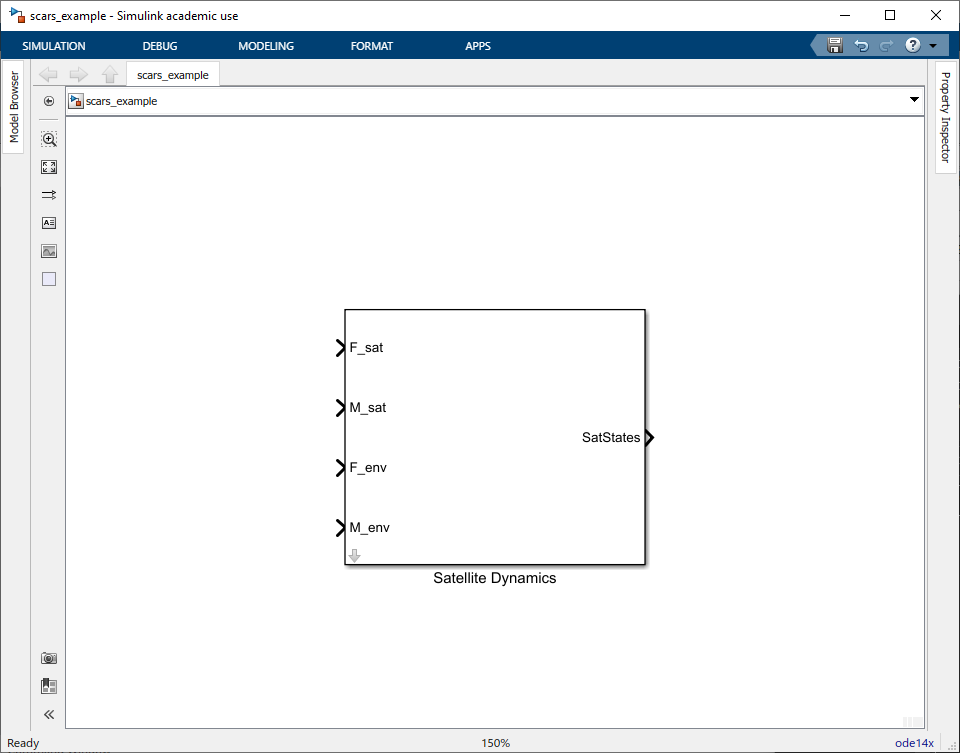
\includegraphics[scale=0.41]{4-examples/01a.png}\label{sub:01a} }}%
                \qquad
                \subfloat[Spacecraft Dynamics Mask]{{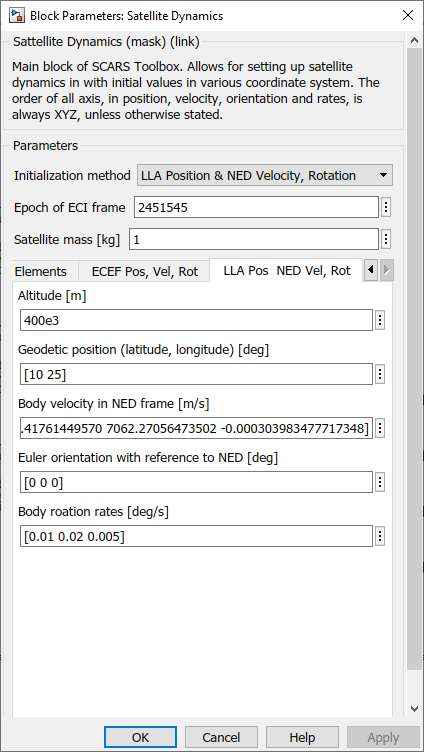
\includegraphics[scale=0.41]{4-examples/01b.png}\label{sub:01b} }}%
                \caption{Step 1}%
                \label{fig:step1}%
            \end{figure}

            To set up the spacecraft as a point in orbit spacecraft dynamics model everything that needs to be done is to add \textbf{Spacecraft Dynamics} block from \ac{scars} Parts Library, as seen on \autoref{fig:step1} \subref{sub:01a} and to input parameters describing the simulated spacecraft into object's mask. Available are several initialization methods, corresponding to reference frames in which the user can input the starting point. In this case, since the objective is to track geographic coordinates, the method of choice is \textbf{LLA Position \& NED Velocity, Rotation}. The choice of parameters, corresponding to average CubeSat, can be seen on Figure \autoref{fig:step1} \subref{sub:01b}. Initial latitude and longitude were chosen arbitrarily and are in the neighborhood of the tracking point, which will be set up later.
            
            Afterwards the user can set up Simulink model solver parameters to \textbf{Fixed-step} with \textbf{ode14x} solver choice, with the rest left to default settings. It is not necessary, but allows for larger step-size when using \textbf{Derivative} blocks.
            % the screenshot filled \textbf{Spacecraft Dynamics} Simulink mask.

        \subsubsection*{Step 2: Environment setup}
            \begin{figure}[H]
                \centering
                \subfloat[Example Model]{{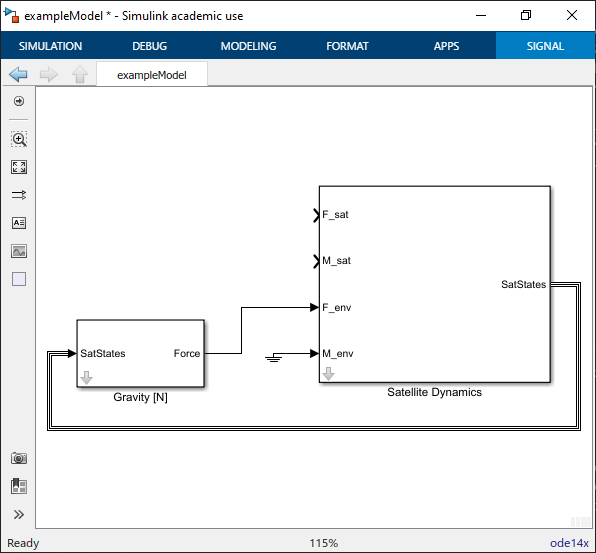
\includegraphics[scale=0.41]{4-examples/02a.png}\label{sub:02a} }}%
                \qquad
                \subfloat[Gravity Mask]{{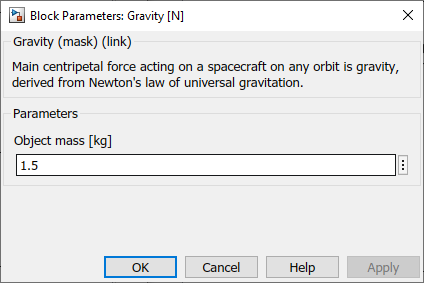
\includegraphics[scale=0.41]{4-examples/02b.png}\label{sub:02b} }}%
                \caption{Step 2}%
                \label{fig:step2}%
            \end{figure}

            As this spacecraft does not use magnetorquers nor does not have any major drag-inducing components, the only relevant block representing environment's influence on the satellite is the \textbf{Gravity [N]} block. The only parameter to input is spacecraft's mass, as seen on \autoref{fig:step2} \subref{sub:02a}.

        \subsubsection*{Step 3: Actuators choice and setup}
            \begin{figure}[H]
                \centering
                \subfloat[Example Model]{{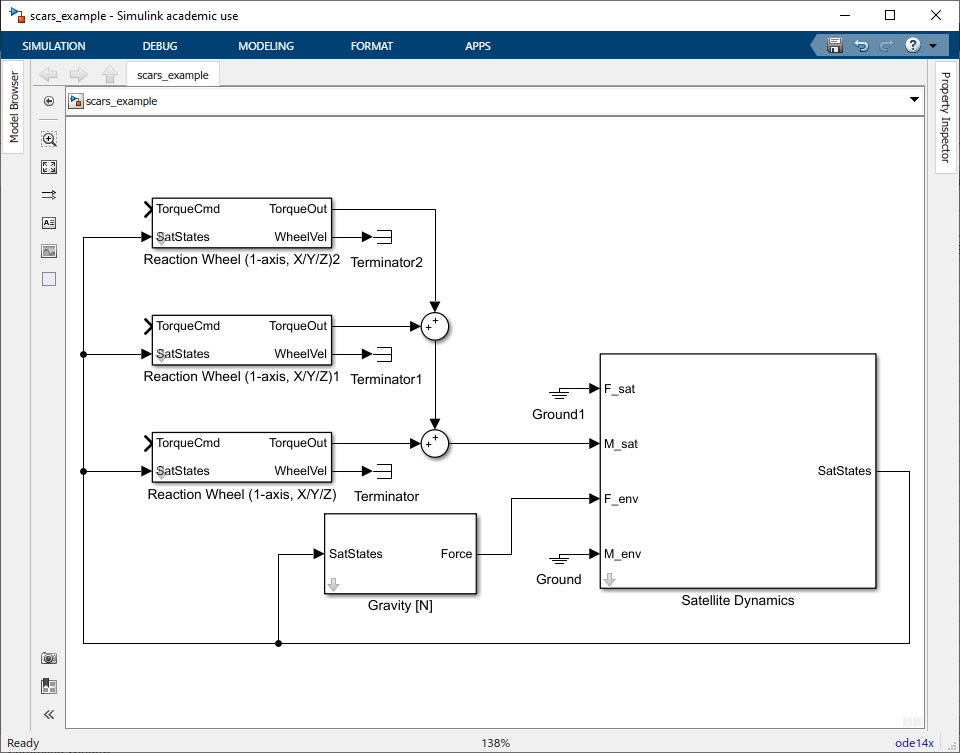
\includegraphics[scale=0.41]{4-examples/03a.png}\label{sub:03a} }}%
                \qquad
                \subfloat[Reaction Wheel Mask]{{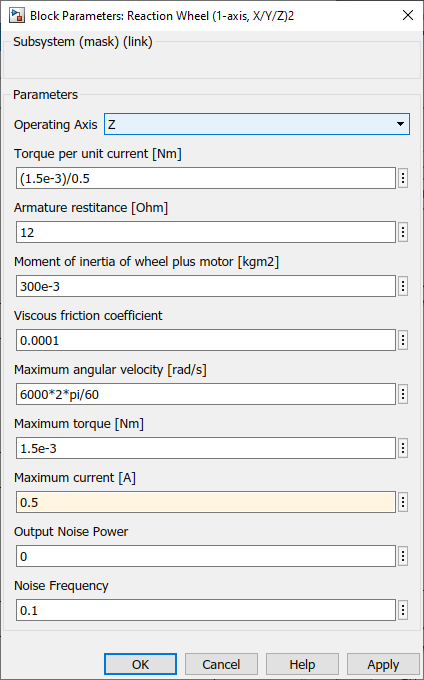
\includegraphics[scale=0.41]{4-examples/03b.png}\label{sub:03b} }}%
                \caption{Step 3}%
                \label{fig:step3}%s
            \end{figure}

            The next step would be to implement the choice of actuators into the spacecraft model. In this example the user could want to test the NanoTorque GSW-600 reaction wheels, in nominal configuration of one wheel for each spacecraft body axis, from GomSpace manufacturer. The list of relevant parameters, compiled from the actuator's datasheet, can be seen on \autoref{fig:step3} \subref{sub:03b}. They were put into as parameters of \textbf{Reaction Wheel (1 axis X/Y/Z)} block from \ac{scars} Parts Library and added to Example Model. The required inputs are the control signal and \textbf{SatStates} bus signal (described in \autoref{sec:space_mechanics}), while the outputs are torque and wheel angular rate.

            % here be table with citation to the datasheet
        
        \subsubsection*{Step 4: Setup of control algorithm}
            \begin{figure}[H]
                \centering
                \subfloat[Example Model]{{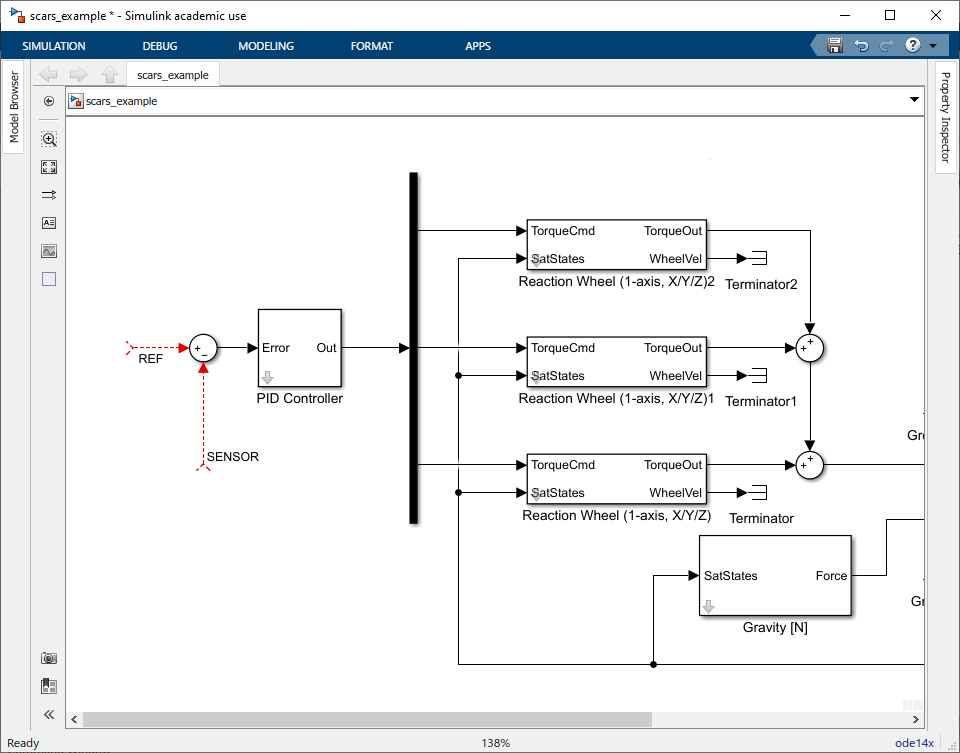
\includegraphics[scale=0.4]{4-examples/04a.png}\label{sub:04a} }}%
                \qquad
                \subfloat[PID Mask]{{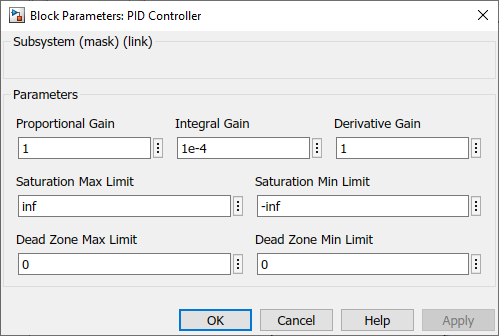
\includegraphics[scale=0.40]{4-examples/04b.png}\label{sub:04b} }}%
                \caption{Step 4}%
                \label{fig:step4}%
            \end{figure}
            A \ac{pid} controller was chosen as a control mechanism as the source of input signal in reaction wheels. The parameters were initially set as can be seen on \autoref{fig:step4} \subref{sub:04b}. Saturation of \textbf{PID Controller} block output signal was set up in accordance to hardware's maximum voltage.

        \subsubsection*{Step 5: Coordinate transformation and reference signal}
            \begin{figure}[H]
                \centering
                \subfloat[Example Model]{{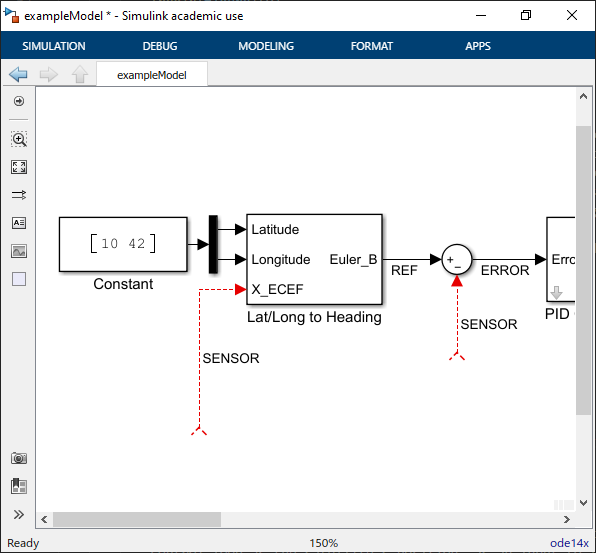
\includegraphics[scale=0.41]{4-examples/05a.png}\label{sub:05a} }}
                \caption{Step 5}%
                \label{fig:step5}%
            \end{figure}
            \ac{scars} Toolbox also provides a way to speed up the process of building mathematical transformations, allowing the user conduct initial tests first and only later think about software implementation. This approach may lead to significant savings in manhours, as failing approaches can be rejected without spending time on setting up algorithms from scratch. In this case, \textbf{Lat/Long to Heading} block was used, without the need for any further setup. As first two inputs are the desired geographical coordinates and the last one is the position vector of the satellite, in \ac{ecef} reference system. 

        \subsubsection*{Step 6: Sensors choice and setup}
            \begin{figure}[H]
                \centering
                \subfloat[Example Model]{{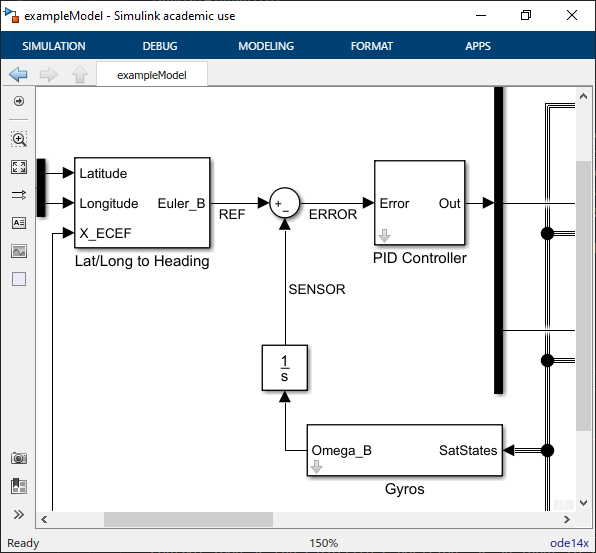
\includegraphics[scale=0.41]{4-examples/06a.png}\label{sub:06a} }}%
                \qquad
                \subfloat[Gyros Mask]{{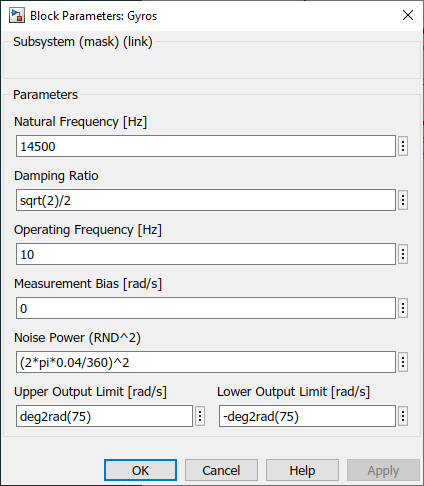
\includegraphics[scale=0.41]{4-examples/06b.png}\label{sub:06b} }}%
                \caption{Step 6}%
                \label{fig:step6}%
            \end{figure}
            As one can see on Figure \dots, the only signals necessary to close the control loop are satellite's position, as an input to \textbf{Lat/Long to Heading} and Euler angles in body reference frame. The former was not relevant to the posed objective of this Example Model, therefore was set up to be measured by the \textbf{Ideal Position Sensor (ECEF)} block, but the latter had to be a gyroscope. \textbf{Gyros} block was added to the simulation and set up with the parameters of the gyroscope, chosen by the fictitious user to be ADXRS614 MEMS Gyroscope, as proposed by Li et al.\cite{li2013design} 
            
            The extract from the datasheet and it's representation as \ac{scars}' block parameters can be found on Figure \autoref{fig:step6} \subref{sub:06a} and \autoref{fig:step6} \subref{sub:06b} respectively.

        \subsubsection*{Step 7: Simulation and verification}
            Finally, the simulation can be run by the user and the results can be verified.         
            \begin{figure}[H]
                \centering
                \subfloat[Example Model]{{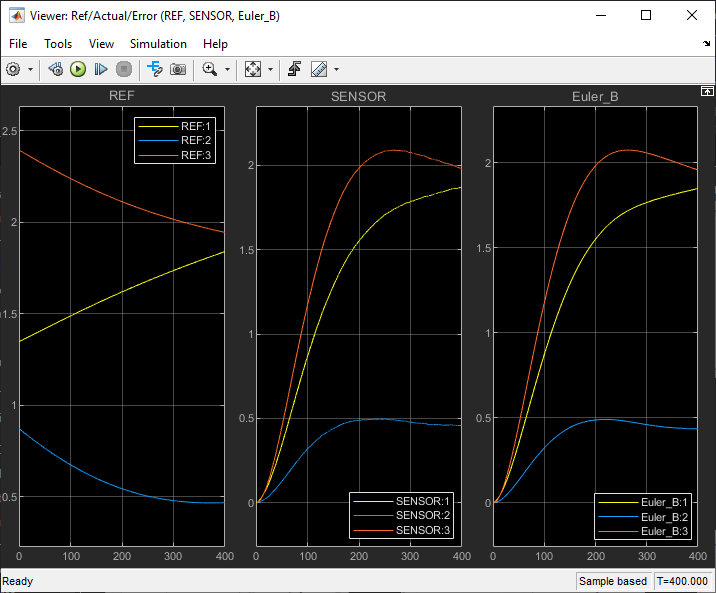
\includegraphics[width=\textwidth]{4-examples/07a.png}\label{sub:07a} }}%
                \caption{Step 7}%
                \label{fig:step6}%
            \end{figure}
 
            \dots\textit{finish description}\dots

    \subsection{PW-Sat2}
        % Magnetorquers
        As written on its website, "PW-Sat2 is a student satellite project started in 2013 at Warsaw University of Technology by the Students Space Association members. Its main technical goal is to test new deorbitation technology in form of a large deorbitation sail whereas the project purpose is to educate a group of new space engineers. In February 2018 PW-Sat2 became fully integrated and was being prepared to the launch into orbit planned for the second half of 2018."\cite{pwsat2website}
        % https://pw-sat.pl/wp-content/uploads/2014/07/PW-Sat2-C-01.00-ADCS-CDR.pdf
        
        \dots\textit{screenshots of model}\dots

        \subsubsection{Detumbling}
            One of two modes of control that PW-Sat2 operates in (with the other one being Sun Pointing Mode) is Detumbling Control Mode. Detumbling maneuver is performed after deployment of the spacecraft from a carrier rocket. As the satellites are separated from the deployment mechanism, they are burdened by non-zero initial angular rates. To counteract that and stabilize a satellite PW-Sat2 is equipped with a set of two perpendicular magnetorquer rods and one air core, in total one coil acting along each of satellite's body axis. The most important parameters used by \ac{scars} model of PW-Sat2 are listed in Table \ref{table:pwsat2magne}.\cite{pwsat2adcs} Exact values are taken directly from the datasheet of \ac{imqt} \cite{imqt-datasheet}, which is used in PW-Sat2.

                \begin{center}    
                    \small
                    \begin{tabular}{l l}
                        \textbf{Parameter} & \textbf{Value} \\ \hline
                        Nominal magnetic dipole & $0.2 Am^2$ \\
                        Maximum actuation envelope error & $3\mu T$ \\
                        Power consumption during actuation & $1.2W$ \\
                        Mass & 196g
                    \end{tabular}
                \end{center}\label{table:pwsat2magne}

                \dots\textit{plots with description}\dots

        \subsubsection{Deorbitation with drag sail}
            One of the main objectives of PW-Sat2 mission was to deploy and test the effectiveness of it's drag sail in deorbitation maneuver. The sail was  $2$x$2m$ square made from aluminized polyester boPET film\cite{pwsat2dt}.
            
            In this example, \ac{scars} toolbox was tested against data points derived from NORAD measurements. The simulation was run in two cases: only with drag sail set up and with drag sail and magnetorquers on to keep sail's plane perpendicular to spacecraft's orbit tangent vector. The sail was deployed around 25th day of the mission.
                         
            \begin{figure}[H]
                \centering
                \includegraphics[width=1\textwidth, height=160px]{example-image-a}
                \caption{Results from \ac{scars} simulation, with only drag sail included}
                \label{fig:scars-deorbit}
            \end{figure}

            It is visible on \autoref{fig:pw-sat-deorbit} that since deployment moment satellite's altitude began decreasing, showing the negative effect of drag sail on body's velocity. When compering results from \ac{scars} simulation with data collected from PW-Sat2 \ac{tle}s, presented on \autoref{fig:pw-sat-deorbit} it is apparent that attitude changes are much more drastic in \ac{scars} model than in real life. This is an expected result, as in PW-Sat2, shortly after deployment the sail has torn, therefore the effective drag was much lower than simulated value. 
            
            \begin{figure}[H]
                \centering
                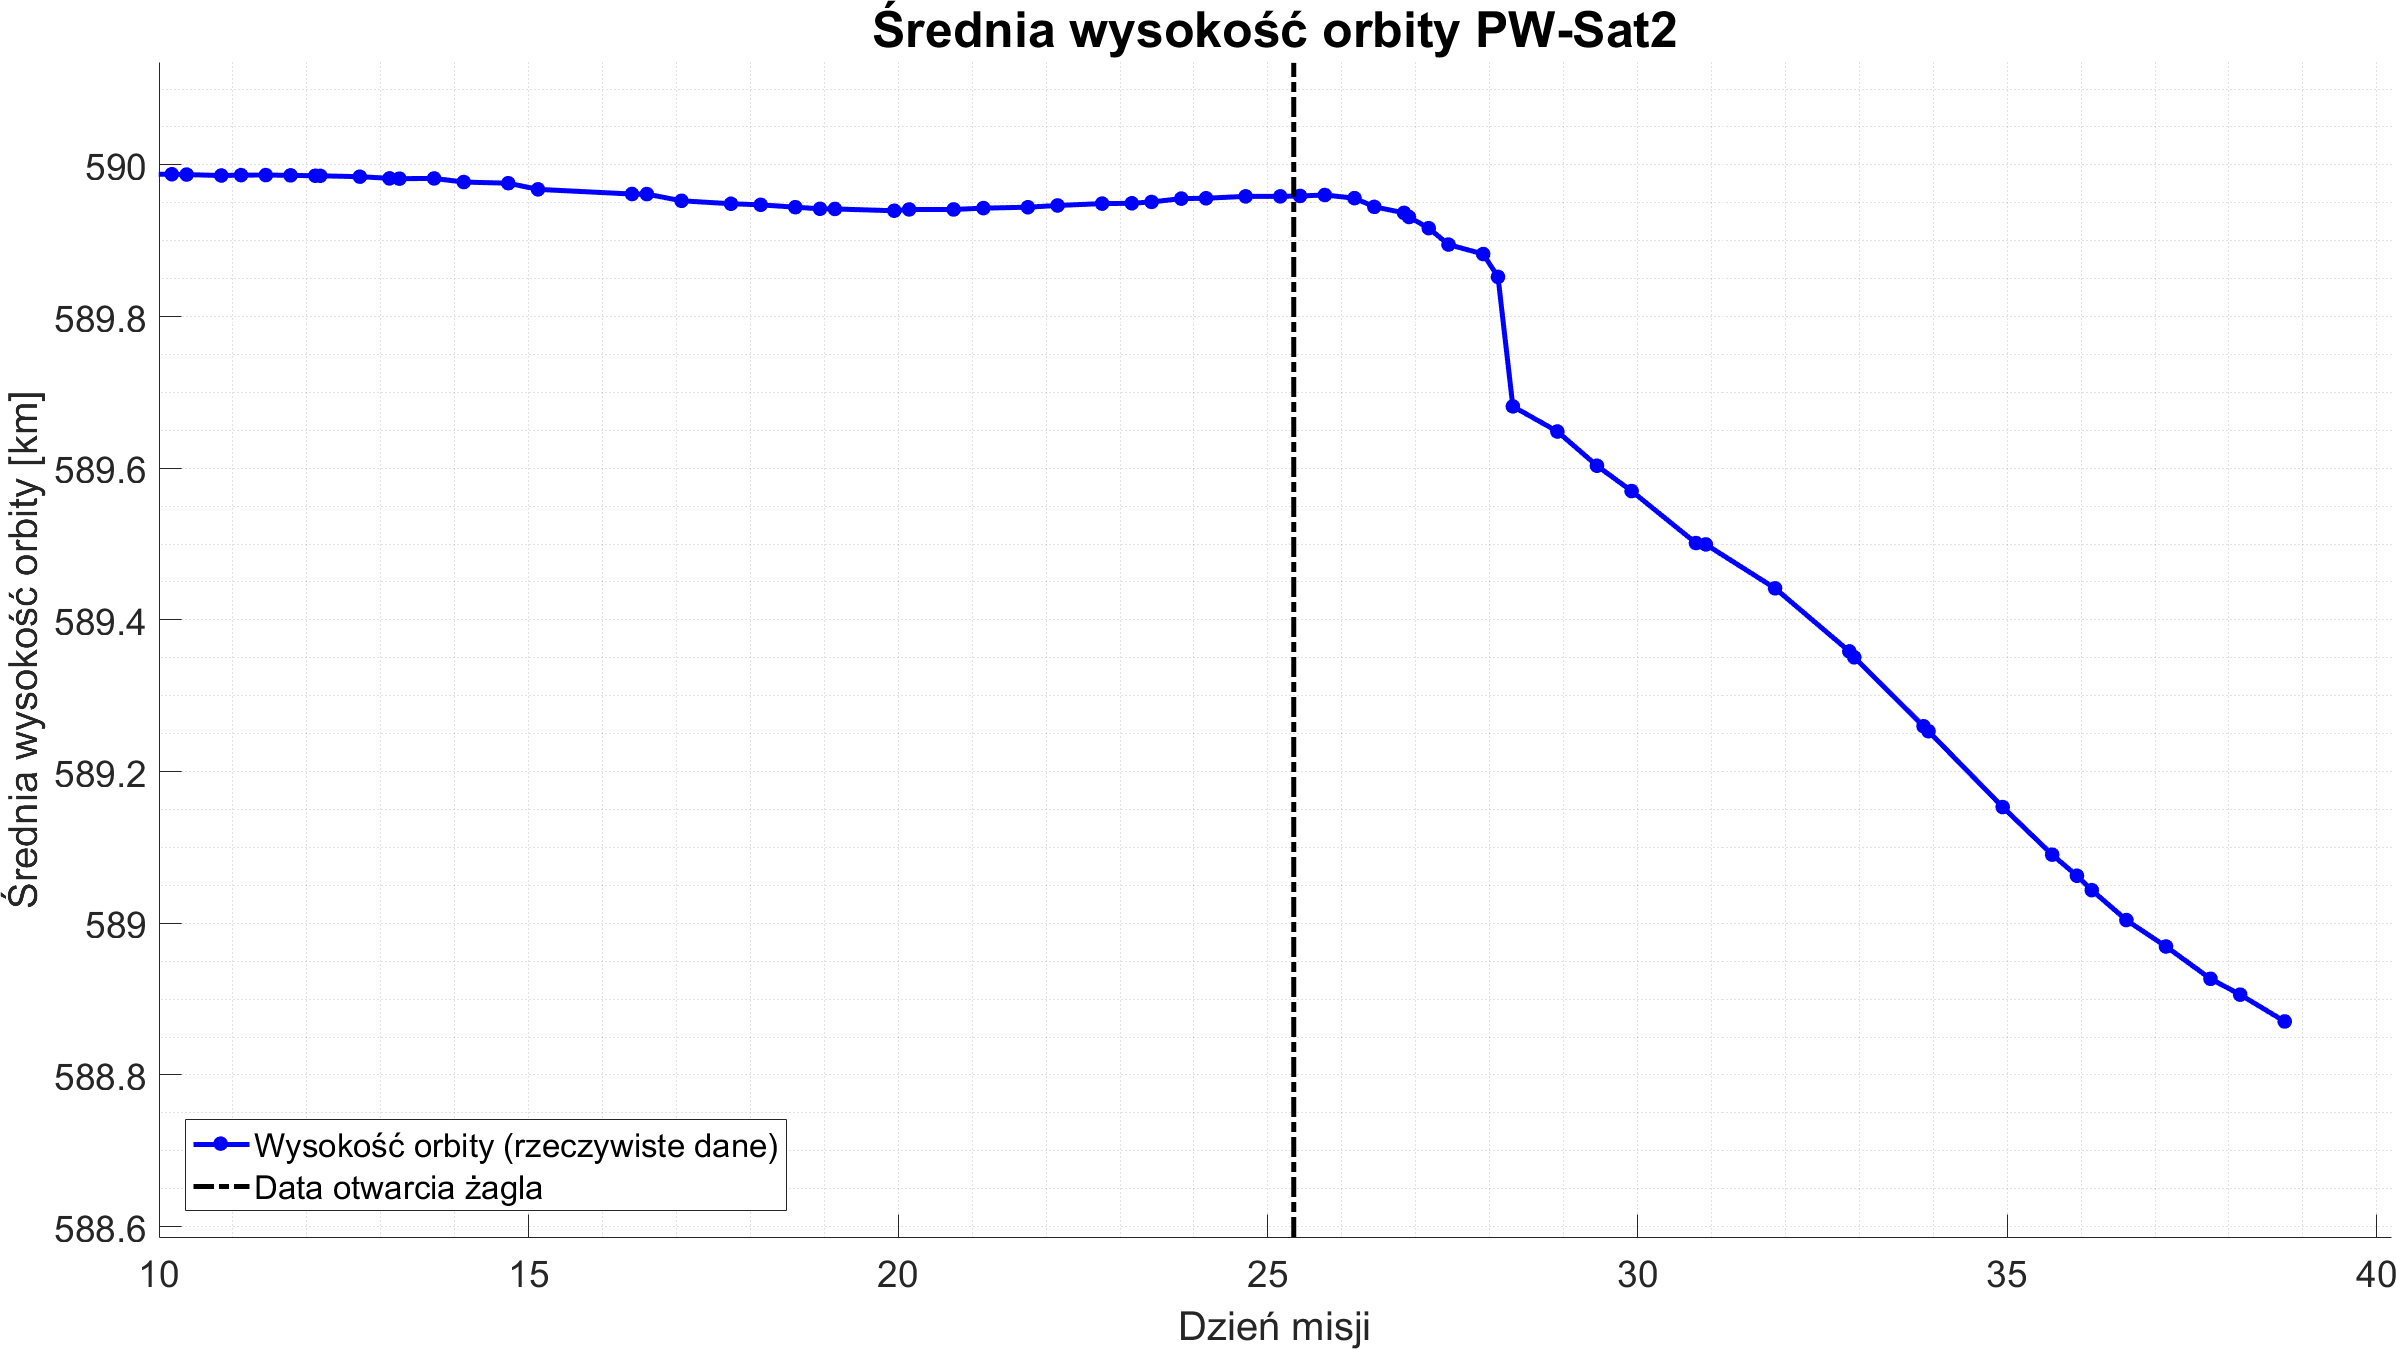
\includegraphics[width=1\textwidth]{4-examples/pw-sat-deorbit.png}
                \caption{Average altitude of PW-Sat2 satellite as taken from NORAD measurements. On X axis there is mission time in days, on Y axis there is average altitude in km.}
                \label{fig:pw-sat-deorbit}
            \end{figure}
            
            \begin{figure}[H]
                \centering
                \includegraphics[width=1\textwidth, height=160px]{example-image-b}
                \caption{Results from \ac{scars} simulation, with magnetorquer-driven attitude correction}
                \label{fig:scars-deorbit3}
            \end{figure}


        % \subsubsection{PROBA-1}
        % https://directory.eoportal.org/web/eoportal/satellite-missions/p/proba-1#spacecraft


    \subsection{Sentinel-2} 
    
    Sentinel-2 is a European polar satellite mission carried out by \ac{esa} as a part of Copernicus Programme. It consists of constellation of twin polar orbit satellites, Sentinel-2A and Sentinel-2B and it's aim is to deliver Earth observation data to broad public, providing wide range of services such as natural emergency management, agricultural monitoring or water classification  \cite{sentinelreference_description}.

    As per document describing Sentinel-2 \ac{adcs} subsystem, the satellites operate on a sun-synchronous orbit, with $786km$ mean altitude and $10:30$ local time of descending node. They maintain Earth-oriented attitude in all operational modes. The required pointing performance is moderate, but the main design driver is the need for precise geo-location of the images \cite{sentinelreference_adcs}.

    The actuators on board of Sentinel-2 and simulated with \ac{scars} toolbox for demonstration purposes are described in Table \ref{table:sentinel-adcs}.

    % Gyro: https://spaceequipment.airbusdefenceandspace.com/avionics/fiber-optic-gyroscopes/astrix-200/
    % Thrusters: https://www.yumpu.com/en/document/read/10860453/1-n-monopropellant-thruster-astrium-st-eads
    % Magnetometer: http://www.zarmtec.uni-bremen.de/products/magnetometer/
        
    \begin{center}    
        \small
        \begin{tabularx}{\textwidth}{ c l X l l }
            \textbf{No.} & \textbf{Uni}t & \textbf{Type} & \textbf{Supplier} & \textbf{Name} \\ \hline
            3 & MAG & 3-axis fluxgate magnetometer & ZARM Technik & FGM-A-75 \\
            2 & GPRS & 2 band GPS receiver & RUAG & - \\
            3 & STR  & Active pixel sensor star tracker & Jena Optronik & Astro APS \\
            4 & IMU & High performance fibre optical gyro & Astrium & ASTRIX 200 \\
            3 & MTQ & $140 Am^2$ magnetic torquer & ZARM Technik & MT140-2\\
            4 & RW & $18 Nms$ reaction wheel & Honeywell & HR12 \\
            8 & THR & $1N$ monopropellant thruster & EADS ST &CHTIN-6
        \end{tabularx}
    \end{center}\label{table:sentinel-adcs}

    \dots\textit{earth-pointing test: plots and description}\dots

\subsection{Examples of tests possible with SCARS}
    \dots\textit{introduction}\dots

    \subsubsection{Control system robusntess analisys}
    
        \dots\textit{plots and description}\dots
        

    \subsubsection{Long term simulation}
        \dots\textit{plots and description}\dots

    \subsubsection{Contingency scenarios}
        \ac{scars} provides an easy ways of testing various contingency scenarios, which means it is possible to quickly adapt the simulation to represent redundant structures, by swapping one sensor or actuator for another, or even by just modifying existing elements. Scenario and Example Model from \autoref{sec:simple_spacecraft} can be given as a good example. In this case,  Nan-oTorque GSW-600 reaction wheels set contains four reaction wheels, one for each Cartesian axis and one on located on direction vector $\textbf{r} = [1 1 1]$, which makes it possible to have 3 degrees of freedom even if one actuator is not responding.

        To adapt Example Model to this scenario, one must only change one reaction wheel block from \textbf{Reaction Wheel (1-axis, X/Y/Z)} to \textbf{Reaction Wheel (1-axis, vector)} and set the \textbf{Operating Axis} parameter to $[1 1 1]$ value (the norm calculated from the vector, so it's length is not relevant).


        \dots\textit{plots and description}\dots
